


\chapter{Εισαγωγή στα Ασύρματα Δίκτυα Αισθητήρων}

\section{Εισαγωγή}
Στα τέλη της δεκαετίας του 1990 αναπτύχθηκαν στον κόσμο των υπολογιστών και της πληροφορικής, αμφότερα τα όραματα "Περιρρέουσα Νοημοσύνη" ( Ambient Intelligence ) και
του "Διάχυτου Υπολογισμού" (Pervasive Computing ή πιο συχνά Ubiquitus Computing).
Η έννοιες αυτές αναφέρονται αφηρημένα σε ένα περιβάλλον το οποίο είναι ικανό να "νιώθει" και να καταλαβαίνει τους ανθρώπους, και γενικότετερα
τις οντότητες, που βρίσκονται σε αυτό \cite{ambient}.
Λίγο πιο συγκεκριμένα, σε ένα τέτοιο περιβάλλον υπάρχουν αυθαίρετα πολλές συσκευές οι οποίες επικοινωνούν και συνεργάζονται μεταξύ τους με κοινό στόχο την εξυπηρέτηση
του ανθρώπου.
Η εξυπηρέτηση αυτή έχει να κάνει από τις καθημερινές εργασίες, όπως αυτόματος οπλισμος/αφοπλισμός συναγερμού, αυτόματο πότισμα, αυτόματο άνοιγμα των φώτων, παράθυρων
και ρύθμιση της θερμοκρασίας του σπιτιού όταν εισέρχεται ο ιδιοκτήτης του, αλλά και πιο προηγμένες τεχνολογιές όπως αντιμετώπιση μιας πυρκαγιάς σε ένα δημόσιο κτήριο
ή υπόδειξη νέων κατάλληλων
προιόντων σύμφωνα με τις καταναλωτικές συνήθειες μιας οικογένειας.

Γίνεται επομένως εμφανές οτι το όραμα αυτό, αν και αρκετά ελπιδοφόρο, στην τελική του μορφή περιλαμβάνει πολλές τεχνολογίες και επιστήμες μαζί, αποτελεί δηλαδή ένα
σχετικά καινούργιο διεπιστημονικό πεδίο.
Συγκεκριμένα για την υλοποίηση του οράματος χρειάζονται βασικά εργαλεία (γνώσεις και αλγόριθμοι) από επιστήμες όπως η Θεωρία Πληροφορίας, της Ανοχής σε Σφάλματα,
τα Δίκτυα, τα Ασύρματα Κινητά Δίκτυα, τα Ασύρματα Δίκτυα Αισθητήρων, τα Κατανεμημένα Συστήματα, της Ασφάλειας και πολλών άλλων. Ένας παραστατικός συνδυασμός αυτών
των επιστημών με τελικό αποτέλεσμα αυτών τον Διάχυτο Υπολογισμό φαίνεται στην εικόνα \ref{fig:pervasive}.

\begin{figure}
	\centering
	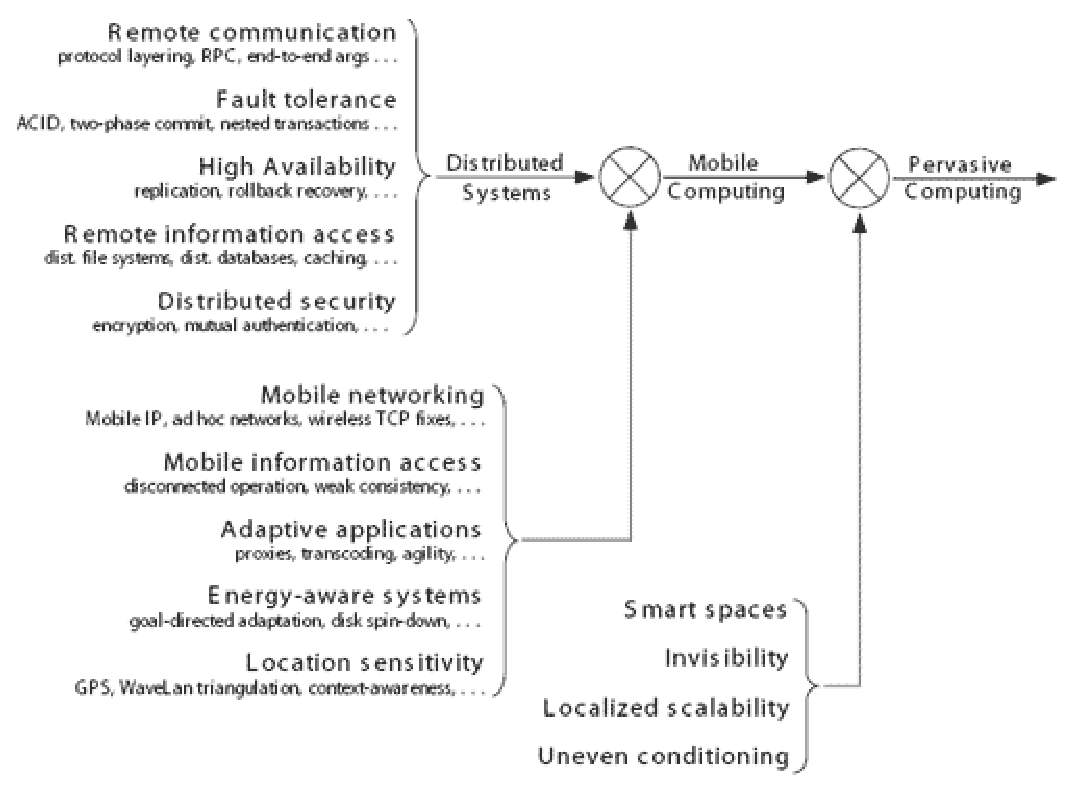
\includegraphics[width=0.8\textwidth]{images/pervasive_computing.eps}
  \caption[Caption for LOF]{Ο Διάχυτος Υπολογισμός ως συνδυασμός επιστημών\footnotemark}
	\label{fig:pervasive}
\end{figure}

Ένα από τα πιο σημαντικά, αν όχι το πιο σημαντικό, εργαλεία του Διάχυτου Υπολογισμού είναι τα Ασύρματα Δίκτυα Αισθητήρων(ΑΔΑ).
Τα ΑΔΑ αποτελούνται από έναν μεγάλο αριθμό κόμβων οι οποίοι καλύπτουν επαρκώς το περιβάλλον το οποίο είναι σε επιτήρηση.
Είναι το υποσύστημα το οποίο καταγράφει όλες τις πληροφορίες από το περιβάλλον αλλά και ταυτόχρονα είναι το ίδιο υποσύστημα που εκτελεί τις λειτουργίες που είναι
απαραίτητες κάθε στιγμή.
Ένα από τα κρισιμότερα συστατικά των ΑΔΑ είναι ο αισθητήρας: είναι το υποσύστημα του κόμβου το οποίο μετατρέπει μια φυσική ποσότητα όπως η υγρασία, η θερμοκρασία
κλπ σε ηλεκτρονικό δεδομένο.
Η επιστημονική κοινότητα από τις αρχές του 2000, αφού έχει μελετήσει σε βάθος τις προηγούμενες επιστήμες, σε σχέση με τα ΑΔΑ, όπως τα Δίκτυα, Ασύρματα Δίκτυα,
Κατανεμημένα Συστήματα κλπ έχει εστιάσει μεγάλο μέρος της προσοχή της στα Ασύρματα Δίκτυα Αισθητήρων αφού αποτελούν απαραίτητο εργαλείο για τον Διάχυτο Υπολογισμό.

\footnotetext{Η εικόνα παρουσιάζεται στην ιστοσελίδα του εργαστηρίου Διάχυτου Υπολογισμού του πανεπιστημίου Carnegie Mellon (CMU)}

Τα τελευταία αυτά 10 χρόνια, τα Ασύρματα Δίκτυα Αισθητήρων γνώρισαν τρομερή πρόοδο σε όλο το διάστημα. Εφευρέθηκαν μαθηματικά μοντέλα που προσομοιώνουν πλήρως τα
ΑΔΑ\cite{geometric_graphs}, αλγόριθμοι οι οποίοι εκμεταλεύονται πλήρως τις ιδιότητές τους ώστε να έχουν καλύτερη απόδοση, άνω και κάτω φράγματα σε αποδόσεις
αλγορίθμων και πολλά άλλα.
Ο πιο σημαντικός περιορισμός τους, ο οποίος διαπιστώθηκε από την αρχή της έρευνας, είναι οι περιορισμένοι πόροι των κόμβων ειδικά σε θέματα ενέργειας.
Η περιορισμένη χωρητικότητα ενέργειας ενός κόμβου είναι το σημείο κλειδί το οποίο μάλιστα διαφοροποιεί τα ΑΔΑ από τα κλασσικά Ασύρματα Δίκτυα.
Επομένως η περισσότερη έρευνα πανω στα ΑΔΑ, ακόμα και 10 χρονια μετά, έχει σχέση με την ελαχιστοποίηση της κατανάλωσης της ενέργειας. Είναι πλέον αποδεκτό οτι με την
σημερινή τεχνολογία τα ΑΔΑ δεν γίνεται να λειτουργούν επ'άπειρον χωρίς την ανθρώπινη παρέμβαση κάτι που επηρεάζει σημαντικά το όραμα του Διάχυτου Υπολογισμού.
Διότι αν ο κάθε κόμβος σε ένα ΑΔΑ χρειάζεται ανθρώπινη παρέμβαση ανά τακτά χρονικά διαστήματα τότε το κόστος του συνολικού συστήματος αυξάνεται σημαντικά, ένας τομέας
που από την έναρξη μαζικής παραγώγής τέτοιων συστημάτων λαμβάνεται σοβαρά υπόψη και καθορίζει τελικά την επιτυχία τους. Όμως ακόμα και αν εξαιρέσουμε τον παράγοντα
του κόστους, ένα ΑΔΑ στο οποίο οι κόμβοι λόγω περιορισμένης ενέργειας διακόπτουν τη λειτουργία τους απρόσμενα μετά το ίδιο το δίκτυο γίνεται αναξιόπιστο
αποτυγχάνοντας τον αρχικό του στόχο: να βοηθά τον άνθρωπο.

Ωστόσο μια καινούργια τεχολογία που εφευρέθηκε από τους επιστήμονες του MIT \cite{power_mit_1} έρχεται να αλλάξει άρδην τις προσδοκίες στο πεδίο των ΑΔΑ. Η τεχνολογία
αυτή επιτρέπει την ασύρματη μετάδοση ενέργειας από μια πηγή σε έναν δέκτη με πολύ μικρές απώλειες ενέργειας. 






\section{Ασύρματα Δίκτυα Αισθητήρων(ΑΔΑ)}
Ένα Ασύρματο Δίκτυο Αισθητήρων(ΑΔΑ) αποτελείται από αυτόνομους κατανεμημένους κόμβους(ή αισθητήρες) όπου ο καθένας λαμβάνει μετρήσεις για το κοντινότου περιβάλλον,
όπως θερμοκρασία, υγρασία, επίπεδα θορύβου, σεισμικές δονήσεις, πίεση ακόμα και κίνηση με την προϋπόθεση πάντα οτι υπάρχει το απαραίτητο υλικό πάνω στον κόμβο ωστε
να μπορεί να λάμβάνει εκάστοτε μέτρηση.
Οι κόμβοι λαμβάνουν μετρήσεις περιοδικά με περίοδο που εξαρτάται από το είδος το δικτύου και ρυθμίζεται από τον αρχικό σχεδιαστή του δικτύου.
Για ένα δίκτυο οι κόμβοι μπορεί να λαμβάνουν μετρήσεις ανά μια ώρα ενώ σε κάποιο άλλο δίκτυο οι αισθητήρες μπορεί να λαμβάνουν μετρήσεις ανα ένα δευτερόλεπτο.
Σε ένα ΑΔΑ σχεδόν πάντα θεωρείται οτι υπάρχει ένα ακόμα πολύ σημαντικό στοιχείο: η Πηγή.
Ο κάθε κόμβος αφού λάβει και καταγράψει ένα μέγεθος μετρήσεων στέλνει τα δεδομένα αυτά, δομημένα σε πακέτα μέσα από ένα πρωτόκολλο δρομολόγησης, στην Πηγή
χρησιμοποιώντας ως διαμελοσαβητές άλλους κόμβους.
Θα πρέπει να αναφερθεί οτι ο κάθε κόμβος δεν γνωρίζει την συνολική διαδρομή που θα ακολουθήσουν τα πακέτα αλλά γνωρίζει μόνο τον πρώτο γείτονα στον οποίο στέλνει κάθε
φορά ένα πακέτο που έχει προορισμό την Πηγή. 

Τα βασικά κριτήρια που χαρακτηρίζουν ένα δίκτυο ως ΑΔΑ είναι τα εξής:
\begin{itemize}
\item μεγάλοι περιορισμοί ως προς την κατανάλωση ενέργειας για τους κόμβους
\item ικανότητα του δικτύου να μπορεί να αντιμετωπίζει αποδοτικά δυσλειτουργίες και σφάλματα κόμβων
\item ικανότητα αντιμετώπισης αποτυχιών και προβλήματα επικοινωνίας μεταξύ κόμβων
\item ανομοιογένεια ως προς τους κόμβους
\item τοπικότητα στην πληροφορία
\item επεκτασιμότητα του δικτύου σε πολύ μεγάλα μεγέθη
\item εύκολη εγκατάσταση και χρήση του συνολικού δικτύου από έναν χειριστή
\end{itemize}
Ο αριθμός των κόμβων μπορεί να κυμαίνεται από μερικές εκατοντάδες μέχρι και αρκετές χιλιάδες.
Η κατανομή των κόμβων, δηλαδή ο τρόπος που τοποθετούνται, συνήθως είναι ομοιόμορφη αλλά αυτό δεν ισχύει πάντα. Για παράδειγμα έχει αποδεχτεί οτι μια διαφορετική
κατανομή όπως η Gaussian μπορεί να έχει καλύτερη απόδοση σε ένα ΑΔΑ, όσον αφορά κάποια συγκεκριμένα χαρακτηριστικά \cite{gaussian_sensors}.
Ο κάθε κόμβος αποτελείται συνήθως από κάποια τυπικά μέρη:
\begin{itemize}
\item πομπό/δέκτη που να χρησιμοποιεί χαμηλής ενέργειας ασύρματα πρωτόκολλα
\item μικροελεγκτή χαμηλής κατανάλωσης ενέργειας, από πολύ απλούς των 8bit μέχρι και σύχρονους με μεγάλη υπολογιστική δύναμη. Το κύριο χαρακτηριστικό τους είναι η
μικρή κατανάλωση ενέργειας
\item μπαταρία και γενικά ένας πόρος ενέργειας
\item αισθητήρες όπως θερμόμετρο, βαρόμετρο, κάμερα κλπ
\end{itemize}
Αν και υπάρχει η τεχνολογία να φτιαχτεί το υλικό ενός κόμβου σε μέγεθος "ψείρας", οι μπαταρίες αυξάνουν δραματικά το μέγεθος ούτως ώστε ένας κόμβος να λειτουργεί
απροβλημάτιστα για πλύ καιρό.
Επίσης θα πρέπει να σημειωθεί οτι, αν και θεωρούμε οτι υπάρχουν κάποιοι περιορισμένοι πόροι όσον αφορά το υλικό όπως για παράδειγμα τις δυνατότητες
του μικροεπεξεργαστή και κατα συνέπεια του μικροελεγκτή που φέρει ένας κόμβος, στα ΑΔΑ δεν μελετώνται περιπτώσεις όπου οι κόμβοι δεν έχουν έλεγχο της κίνησής τους ή
δεν έχουν καθόλου μνήμη και ικανότητα εκτέλεσης βασικών πράξεων.
Τέτοιες περιπτώσεις υπάγονται σε άλλα μοντέλα όπως τα πρωτόκολλα πληθυσμών \cite{population_protocols}.

Η Πηγή είναι ένα ξεχωριστό στοιχείο του δικτύου, το οποίο έχει τεράστια υπολογιστική ικανότητα σε σχέση με τους κόμβους, δεν έχει κανέναν περιορισμό πόρων ενώ
ταυτόχρονα έχει εμβέλεια επικοινωνίας
πολύ μεγαλύτερη από τους κόμβους.
Σε μερικά δίκτυα η Πηγή συμμετέχει στο πρωτόκολλο δρομολόγησης ή βοηθάει μερικώς το συνολικό δίκτυο χρησιμοποιώντας τα ιδιαίτερα χαρακτηριστικά της.
Στην Πηγή φθάνουν τελικά όλες οι πληροφορίες και είναι υπεύθυνη για την διαχείρηση αυτών των πληροφοριών όπως για παράδειγμα εκτέλεση ειδικών
ερωτημάτων(queries) επάνω στα δεδομένα για ασφαλή και γρήγορη εξαγωγή συμπερασμάτων για το δίκτυο.

Τα βασικά Ασύρματα Δίκτυα Αισθητήρων σταματάνε σε αυτό το σημείο.
Ο διαχειρισμός των δεδομένων καθώς και η εξαγωγή μετα-πληροφοριών από αυτά τα δεδομένα κλπ αποτελούν μέρη των διεπιστημονικών πεδίων του Διάχυτου Υπολογισμού και
Περιρρέουσας Νουμοσύνης.
Γίνεται επομένως σαφές λόγω του οτι τα ΑΔΑ αποτελούν το πιο κρίσιμο συστατικό για τις προαναφερθήσες επιστήμες.

Τέλος να σημειωθεί οτι γενικώς στα ΑΔΑ θεωρείται οτι οι αισθητήρες έχουν συνεργατικές τάσεις, δηλαδή συνολικά το δίκτυο έχει κοινό στόχο.
Αντίθετα πολύ σπάνια μελετώνται περιπτώσεις όπου ο κάθε κόμβος κοιτάει μεμωνομένα και εγωιστικά το δικό του συμφέρον.
Η ανάλυση αυτών των περιπτώσεων χρησιμοποιεί συνήθως θεωρία παιγνίων \cite{game_theroy_sensor}, ενώ υποδεικνύει ένα πλήρως ανομοιογενές δίκτυο διαφορετικό από την
αρχική φιλοσοφία των ΑΔΑ.

\section{Το Κίνητρο και Σύντομη Ιστορία των ΑΔΑ}
Το βασικό κίνητρο των ΑΔΑ ήταν κατα κύριο λόγο οι στρατιωτικές εφαρμογές.
Επισκόπηση του πεδίου μάχης, αναγνώριση στόχων, παρακολούθηση και καταγραφή των στρατιωτικών δυνάμεων και των διαθέσιμων πυρομαχικών τους ήταν από τις πρώτες
εφαρμογές που είχαν πυροδοτήση την απόσπαση κονδυλιών, από κυβερνήσεις δυνατών κρατών, για την έρευνα τέτοιων μηχανισμών.
Συγκεκριμένα η πρώτη πραγματική εύρευνα πάνω στα δίκτυα αισθητήρων ξεκίνησε μέσα στην δεκαετία του 1980 στην υπηρεσία του υπουργίου Αμύνης των Η.Π.Α, την DARPA
(Defense Advanced Research Projects Agency).
Η υπηρεσία αυτή ξεκίνησε ένα καινούργιο πρόγραμμα το οποίο λεγόταν Κατανεμημένα Δίκτυα Αισθητήρων (DSN, Distributed Sensor Networks).
Ταυτόχρονα το ARPANET (Advanced Research Projects Agency Network) δίκτυο ήταν πλήρως λειτουργικό με 200 πανεπιστήμια και ερευνιτικά κέντρα συνδεδεμένα.
Η βασική ιδέα των DSN ήταν ένα δίκτυο πολλών κατανεμημένων συνδεδεμένων κόμβοι οι οποίοι συνεργάζονταν μεταξύ τους αλλά ο κάθε κόμβος λειτουργούσε ανεξάρτητος.
Το πρωτόκολλο δρομολόγησης που χρησιμοποιήθηκε βασιζόταν στην μέθοδο της πλημύρας.

Αν συνυπολογισθεί οτι εκείνη την περίοδο δεν υπήρχαν προσωπικοί υπολογιστές, πόσο μάλλον φορητοί υπολογιστές, ενώ το Ethernet μόλις άρχιζε και αποκτούσε φήμη, το
πρόγραμμα DSN ήταν πολύ φιλόδοξο.
Η τεχνολογία για την υλοποίση αυτού του εγχειρήματος είχε βρεθεί σε ένα σχετικά πρόσφατο συνέδριο\cite{1978DSN}.
Ουσιαστικά περιελάμβανε έναν αισθητήρα ήχου, ικανότητα αποστολής και λήψης σημάτων χαμηλής ενέργειας και το απαραίτητο λογισμικού κατανεμημένου χαρακτήρα.
Επιστήμονες από το πανεπιστήμιο Carnegie Mellon (CMU), εστίασαν το ενδιαφέρον τους στη κατασκευή ένός λειτουργικού συστήματος το οποίο θα απευθυνόταν σε τέτοιες
συσκευές, δηλαδή συσκευές συνδεδεμένες σε ένα δίκτυο, στις οποίες υπάρχει εύκολη και ενιαία πρόσβαση στους κατανεμημένους πόρους ενός αξιόπιστου DSN συστήματος.
Το αποτέλεσμα αυτού του συστήματος ήταν να δημιουργηθεί το λειτουργικό σύστημα Mach το οποίο για την εποχή του είχε αρκετά πρωτοπόρα στοιχεία \cite{Mach} ενώ είχε
μάλιστα και κάποια περιορισμένη εμπορική επιτυχία.

Λίγο καιρό αργότερα, επιστήμονες στο πανεπιστήμιο MIT επικεντρώθηκαν στην αναγνώριση (εχθρικών) ελικοπτέρων μέσα από επεξεργασία ακουστικών σημάτων.
Το σύστημα που χρησιμοποιήσαν ήταν μικρόφωνα κατανεμημένα διάσπαρτα σε ένα χώρο τα οποία στέλναν τις πληροφορίες τους σε έναν κεντρικό υπολογιστή.
Χρησιμοποίησαν ευρετικούς αλγόριθμους και τεχνικές ταιριάσματος για να μπορέσουν να πετύχουν αποδεχτά αποτελέσματα στην αναγνώριση ελικοπτέρων.
Επιπλέον επέκτειναν το σύστημα DSN προσθέτοντας αλγόριθμούς για επεξεργασία σημάτων και τεχνικών ταιριάσματος\cite{4789229}.
Για την επίδειξη του συστήματος το εργαστήριο Lincoln στο MIT κατασκεύασε ένα πραγματικό δοκιμαστικό σενάριο για την ακουστική αναγνώριση ελικοπτέρων χαμηλής πτήσης
και αεροπλάνων \cite{aircraft}.
Χρησιμοποιήθηκαν κόμβοι που στην πραγματικότητα ήταν μικρόφωνα τα οποία έστελναν με ασύρματη τεχνολογία τα σήματα ήχου σε 3 σταθερούς υπολογιστές(επεξεργαστής
MC68000, 256KB μήμη και 512ΚΒ κοιμή μνήμη).
Στην εικόνα \ref{fig:lincoln_lab}\cite{lincoln_report} φαίνεται το δοκιμαστικό σενάριο.
Τελικά το συνολικό σύστημα δούλεψε επιτυχώςκαι κατάφερε να εντοπίσει τα χαμηλής πτήσης ελικόπτερα και αεροσκάφη.
\begin{figure}
	\centering
	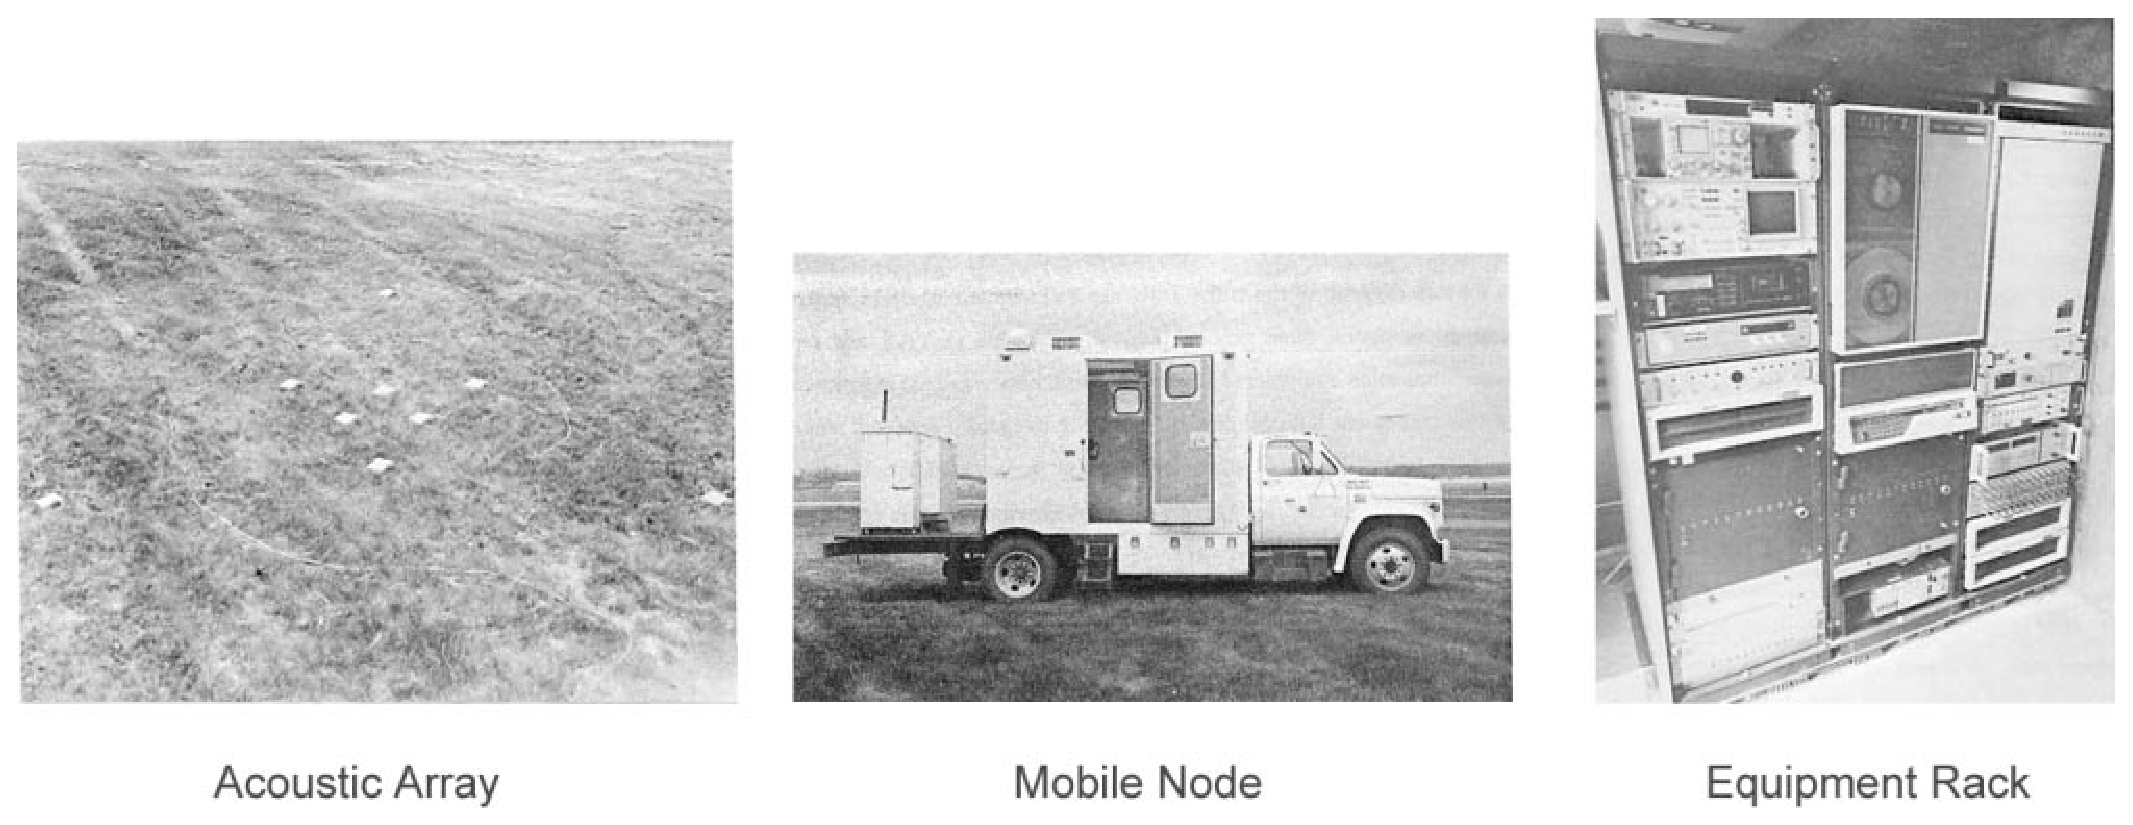
\includegraphics[width=0.8\textwidth]{images/lincoln_lab.eps}
	\caption{Tο δοκιμαστικό πείραμα του εργαστηρίου Lincoln του MIT}
	\label{fig:lincoln_lab}
\end{figure}

Ενώ οι ερευνητές είχαν κατανοήσει οτι τέτοια συστήματα θα έπρεπε να περιλαμβάνουν πολλά μικρά δίκτυα αισθητήρων τα οποία θα έχουν εκατοντάδες κόμβους, η τεχνολογία
για αυτά τα συστήματα δεν ήταν πλήρως έτοιμη.
Ωστόσο στρατιωτικοί παράγοντες είχαν αναγνωρίσει την τεράστια χρησιμότητα αυτών των συστήμάτων καθώς και την υπερτερότητα των δικτυακών όπλων: χιλιάδες αισθητήρες που
συνεργάζονται και μαζεύουν πληροφορίες σε σχέση με τον εχθρό και τις αποστέλλουν στο κέντρο επιχειρήσεων, το οποίο μπορεί να είναι χιλιόμετρα μακριά από το πεδίο
μάχης.
Το προβάδισμα αυτό θα μπορούσε να λειτουργήσει μοιραία στην εξέλιξη μιας μάχης.

Το πρώτο πραγματικό σύστημα που υλοποιήθηκε με αυτόν τον σκοπό και έχει αρκετή σχέση με τα ΑΔΑ είναι το CEC (Cooperative Engagement Capability)\nocite{cec} το οποίο
κατασκευάστηκε από το ναυτικό των Η.Π.Α. στα μέσα της δεκαετίας του 1990.
Το σύστημα αποτελείται από πολλά ραντάρ τα οποία συλλέγουν πληροφορίες για στόχους αέρος όπως αεροσκάφη, ελικόπτερα πύραυλοι κλπ.
Οι μετρήσεις αυτές αποστέλνονται σε έναν κόμβο αρχηγό ( ουσιαστικά πρόκειται για μία Πηγή) ο οποίος επεξεργάζεται και φιλτράρει τις πληροφορίες.
Ο κόμβος αυτός είναι κοινός σε όλους τους άλλους κόμβους που μαζεουν πληροφορίες.
Το σημαντικό στοιχείο του σηστήματος είναι οτι όλοι οι κόμβοι έχουν πρόσβαση σε όλες τις πληροφορές δημιουργώντας ένα πραγματικά κατανεμημνο σύστημα το οποίο δίνει
την ίδια εκόνα σε όλους τους στρατιωτικούς οι οποίοι βρίσκονται σε ένα κόμβο ο καθένας. Το σύστημα αυτό ακολούθησαν και άλλα στρατηγικά συστήματα με παρόμοιους
στόχους όπως το REΒMASS (Remote Battlefield Sensor System) και το TRSS (Tactical RemoteSensor System).


Ταυτόχρονα η τεχνολογία στους υπολογιστές εξελισσόταν ραγδαία.
Είχαν κατασκευαστεί ασύρματα δίκτυα, είχε δημιουργηθεί το Internet, οι μικροεπεξεργαστές είχαν πλέον αρκετή υπολογιστική ισχύ ενώ το υπήρχε η δυνατότητα κατασκευής
μικρουπολογιστικών συστημάτων που είχαν μέγεθος όσο μια παλάμη.
Αυτές οι εξελίξεις σε συνδυασμό με τα οράματα της Περιρρέουσας Νουμοσύνης και του Διάχυτου Υπολογισμού έκαναν τους επιστήμονες να οραματιστούν μια διαφορετική πλευρά
τον δικτύων αισθητήρων: ασύρματα δίκτυα αισθητήρων τα οποία θα συλλέγαν πληροφορίες με στόχο να βοηθήσουν τον άνθρωπο.
Τα ΑΔΑ δηλαδή θα είχαν στόχο να κάνουν πιο εύκολη την ζωή του αθνρώπου από κάθε μεριά αναλαμβάνοντας αυτά κάποιες λειτουργίες σύμφωνα με τις πληροφορίες που έχουν
συλλέξει χωρίς όμως ο άνθρωπος να αλληλεπηδρά με το συνολικό σύστημα.
Έγινε όμως αμέσως αντιληπτό οτι τέτοια συστήματα θα ήταν άμεσα ευπαθή στην διαχείρηση της ενέργειας.
Διότι ενώ όλες οι υπόλοιπες τεχνολογίες είχαν εξελιχθεί ραγδαία, η πρόοδος στις τεχνολογίες της μπαταρίας είχαν πολύ μικρότερη πρόοδο ενώ ταυτόχρονα τέτοια συστήματα
θα έπρεπε να λειτουργούν σχεδόν για πάντα χωρίς την αλληλεπίδραση του ανθρώπου.
Επίσης διαπιστώθηκε οτι αλγόριθμοι για τα κλασσικά ασύρματα δίκτυα (όπως ALOHA, slotted ALOHA κλπ) δεν θα μπορούσαν να χρησιμοποιηθούν καθώς τα ασύρματα δίκτυα έχουν
στόχο την μεγιστοποίηση της απόδοση ενώ τα ΑΔΑ έχουν στόχο την μεγιστοποίηση των χρονικών διαστημάτων που οι κόμβοι, με περιορισμένους πόρους ενέγειας, αποστέλουν
πληροφορίες προς την Πηγή.

Από το 2000 και μετά η προσοχή της επιστημονικής κοινότητας επικεντρώθηκε κυρίως στην ελαχιστοποίηση της κατανάλωσης της ενέργειας στα ΑΔΑ είτε αυτό επιτυγχάνεται
μέσα από τα πρωτόκολλα δρομολόγησης είτε από τον τρόπο ανάπτυξης των αισθητήρων είτε με οποιαδίποτε άλλη τεχνική που θα μπορούσε να κάνει τα ΑΔΑ να αντισταθούν ακόμα
περισσότερη ώρα στο χρόνο.
Επίσης ξεκίνησαν να κατασκευάζονται μαζικά αισθητήρες οι οποίοι ήταν εμπορικά διαθέσιμη για πρακτικούς και ερευνητικούς σκοπός ενώ ταυτόχρονα δημιουργήθηκε το πρώτο
λειτουργικό σύστημα ειδικά για ΑΔΑ, το TinyOS.
Άμεσα οι  πρώτες πειραματικές εφαρμογές που δημιουργήθηκαν με τα ΑΔΑ οι οποίες αφορούσαν σχεδόν όλους τους τομείς της ανθρώπινης δραστηριότητας.

%\begin{comment}
\section{Ασύρματα Δίκτυα Αισθητήρων και οι Εφαρμογές τους}
Η τεχνολογία των Ασύρματων ∆ικτύων Αισθητήρων μπορεί να εφαρμοστεί σε πολλές εφαρμογές του πραγματικού κόσμου και να φέρει στην επιφάνεια κάποιες εντελώς καινούριες.
Ενα κρίσιμο και πρωτεύον συστατικό των κόμβων των ασύρματων δικτύων αισθητήρων είναι ο αισθητήρας.
Για πολλές παραμέτρους του φυσικού περιβάλλοντος υπάρχει η κατάλληλη τεχνολογία αισθητήρα που μπορεί να ενσωματωθεί σε ένα WSN.
Οι πιο ευρέως χρησιμοποιούμενοι είναι οι αισθητήρες θερμοκρασίας, υγρασίας, ήχου, πίεσης και οι χημικοί αισθητήρες.
Μια σύντομη λίστα με τις πιο βασικές εφαρμογές παρουσιάζεται παρακάτω:
\begin{itemize}
	\item \textbf{Πρόληψη Καταστροφών}: Μια από τις πιο συχνά αναφερόμενες εφαρμογές των WSNs είναι στην πρόληψη καταστροφών.
Ένα τυπικό σενάριο για εφαρμογές αυτής της κατηγορίας είναι η ανίχνευση πυρκαγιών.
Οι κόμβοι αισθητήρων είναι εξοπλισμένοι με θερμόμετρα και μπορούν να υπολογίσουν τη θέση τους τρέχοντας κάποιον αλγόριθμο εντοπισμού θέσης (localization).
Τους κόμβους αυτούς μπορούμε να τους απλώσουμε σε ένα δάσος, πετώντας τους από ένα αεροπλάνο. Έτσι σχηματίζεται ένας θερμοκρασιακός χάρτης της
περιοχής και σε περίπτωση υψηλών θερμοκρασιών και χαμηλής υγρασίας που υπονοούν πυρκαγιά ενημερώνουν τους πυροσβέστες.
	\item \textbf{Έλεγχος του περιβάλλοντος και της βιοποικιλότητας} Τα WSNs μπορούν να χρησιμοποιηθούν για να ελέγχουν το περιβάλλον ως προς τους χημικούς ρύπους
ή ακόμα και για το σχηματισμό μιας εικόνας ως προς τον αριθμό των διαφορετικών ειδών πανίδας και χλωρίδας μια περιοχής.
	\item \textbf{Ευφυή Κτίρια} Τα μεγάλα κτίρια συχνά καταναλώνουν μεγάλα ποσά ενέργειας εξαιτίας λανθασμένης χρήσης των συσκευών Air Condtitioning (HVAC).
Μια αποδοτικότερη, πραγματικού-χρόνου και ακριβέστερη παρακολούθηση της θερμοκρασίας, της υγρασίας και άλλων παραμέτρων μπορεί να μειώσει την κατανάλωση ενέργειας.
Επίσης, μπορούν να χρησιμοποιηθούν για την παρακολούθηση των μηχανικών καταπονήσεων σε κτίρια ή γέφυρες που βρίσκονται σε σεισμικά ενεργές Σώνες, ενώ άλλου τύπου
αισθητήρες μπορούν χρησιμοποιηθούν για τον εντοπισμό εγκλωβισμένων ανθρώπων σε περιπτώσεις σεισμού.
Οι αισθητήρες μπορούν να τοποθετηθούν στα κτίρια τη στιγμή της κατασκευής τους ή αφού έχουν κατασκευαστεί.
Σε αυτές τις εφαρμογές η εξοικονόμηση ενέργειας για τους αισθητήρες είναι πολύ σημαντική απαίτηση.
	\item \textbf{∆ιαχείριση Εγκαταστάσεων} Τα WSNs μπορούν να χρησιμοποιηθούν για εφαρμογές διαχείρισης μεγάλων εγκαταστάσεων, όπως θέματα ασφαλείας.
Η είσοδος των ανθρώπων στις εγκαταστάσεις μπορεί να γίνεται χωρίς κλειδιά, αλλά με τη χρήση κάποιου πομπού, ενώ μπορούν να εντοπίζονται πιθανοί εισβολείς.
Επίσης σε χημικές εγκαταστάσεις τα WSNs θα μπορούσαν να χρησιμοποιηθούν για τον εντοπισμό διαρροών.
	\item \textbf{Συντήρηση Μηχανών} Αισθητήρες μπορούν να τοποθετηθούν σε δυσπρόσιτα σημεία μηχανών για να ελέγχουν τους κραδασμούς που υποδεικνύουν ανάγκη για
συντήρηση.
Παραδείγματα τέτοιων μηχανών είναι αυτόματες μηχανές ή οι άξονες των τροχών των τρένων.
	\item \textbf{Εφαρμογές στη Γεωργία} Η εφαρμογή WSNs σε καλλιεργήσιμες εκτάσεις με τοποθέτηση αισθητήρων μέτρησης υγρασίας και ανάλυσης της σύστασης του
εδάφους επιτρέπει την ακριβέστερη και αποδοτικότερη λίπανση και άρδευση των εκτάσεων.
Επίσης, η εκτροφή ζώων μπορεί να ωφεληθεί τοποθετώντας αισθητήρες στα ζώα που ελέγχουν την κατάσταση της υγείας τους.
	\item \textbf{Εφαρμογές στον τομέα της υγείας} Η χρήση WSNs στον τομέα της υγεία μπορεί να αποδειχτεί πολύ ωφέλιμη.
Όμως υπάρχουν αρκετά ηθικά διλήμματα πάνω στο θέμα αυτό.
Οι πιθανές εφαρμογές εκτείνονται από την άμεση τοποθέτηση αισθητήρων στον ίδιο τον ασθενή για την παρακολούθηση της υγείας του και ίσως αυτόματη χορήγηση φαρμάκων,
μέχρι την παρακολούθηση των ιατρών και των ασθενών στα νοσοκομεία.
	\item \textbf{Ευφυή οδικά συστήματα} Στα ευφυή οδικά συστήματα αισθητήρες τοποθετούνται στους δρόμους, ακόμα και στα κράσπεδα των δρόμων οι οποίοι
συλλέγουν πληροφορίες για την κίνηση και την κατάσταση του οδικού δικτύου γενικότερα και επικοινωνούν με τους οδηγούς δίνοντάς τους χρήσιμες πληροφορίες.
	\item \textbf{Στρατιωτικές Εφαρμογές} Τα WSNs μπορούν να είναι ενιαίο και αναπόσπαστο τμήμα των στρατιωτικών συστημάτων.
Τα χαρακτηριστικά των WSNs, όπως είναι η γρήγορη τοποθέτηση τους, η αυτο-οργάνωση και η ανοχή στα σφάλματα, τα μετατρέπουν σε μια πολλά υποσχόμενη τεχνολογία για τα
στρατιωτικά συστήματα.
Κάποιες από τις πιθανές στρατιωτικές εφαρμογές τους είναι η παρακολούθηση της κατάστασης των εξοπλισμών και των πολεμοφοδίων, η στενή παρακολούθηση του πεδίου της
μάχης, η αναγνώριση των εχθρικών δυνάμεων, η εκτίμηση των καταστροφών μετά από μάχη καθώς και ο εντοπισμός και η αναγνώριση χημικής, ατομικής ή βιολογικής επίθεσης.
\end{itemize}




\section{Περιβάλλοντα Ανάπτυξης Εφαρμογών}

\section{Σχεδιασμός Δικτύου και Προκλήσεις}

\section{Τα ΑΔΑ στο Μέλλον}
%this paragraph should end by showing the need for immortal WSNs !!
\section{Επισκόπηση της Διπλωματικής}

%\end{comment}
\label{ch:wsns}